\documentclass[a4paper, 12pt]{article} % Fuente 12pt
\usepackage[utf8]{inputenc}
\usepackage[T1]{fontenc}
\usepackage{hyperref}
\usepackage[left=3cm, right=3cm, top=3.5cm, bottom=3.5cm]{geometry} % Márgenes recomendados
\usepackage{times} % Fuente Times New Romans
\usepackage[english]{babel} 
\usepackage[style=ieee, backend=bibtex]{biblatex} % Bibliografía en formato IEEE
\usepackage{sectsty}
\usepackage{cover}
\usepackage{graphicx}
\graphicspath{ {images/} } % Directorio imágenes
\usepackage{listings} % Formateo código
\usepackage{scrextend}
% Lista de acronimos
\usepackage[acronym]{glossaries}
\makeglossaries
% List of acronyms
\newacronym{ssi}{SSI}{Self-Sovereign Identity}
\newacronym{rpc}{RPC}{Remote Procedure Call}
\newacronym{json}{JSON}{JavaScript Object Notation}
\newacronym{evm}{EVM}{Ethereum Virtual Machine}
\newacronym{w3c}{W3C}{World Wide Web Consortium}
\newacronym{dlt}{DLT}{Distributed Ledger Technology}
\newacronym{baas}{BaaS}{Blockchain as a Service}
\newacronym{aws}{AWS}{Amazon Web Services}
\newacronym{eth}{ETH}{Ether}
\newacronym{eoa}{EOA}{Externally Owned Accounts}
\newacronym{api}{API}{Application Programming Interface}
\newacronym{eth2}{Eth2}{Ethereum 2.0}
\newacronym{rts}{RTS}{Run-Time Systems}
\newacronym{http}{HTTP}{Hypertext Transfer Protocol}
\newacronym{did}{DID}{Decentralized Identifier}
\newacronym{dids}{DIDs}{Decentralized Identifiers}
\newacronym{gdpr}{GDPR}{General Data Protection Regulation}
\newacronym{eidas}{eIDAS}{European system for the recognition of electronic identities}
\newacronym{dif}{DIF}{Decentralized Identity Foundation}
\newacronym{ietf}{IETF}{Internet Engineering Task Force}
\newacronym{oidf}{ODIF}{OpenID Foundation}
\newacronym{jwt}{JWT}{JSON Web Token}
\newacronym{jwts}{JWTs}{JSON Web Tokens}
\newacronym{jws}{JWS}{JSON Web Signature}
\newacronym{jwe}{JWE}{JSON Web Encryption}
\newacronym{mac}{MAC}{Message Authentication Code}


% Copyright 2017 Sergei Tikhomirov, MIT License
% https://github.com/s-tikhomirov/solidity-latex-highlighting/

\usepackage{listings, xcolor}

\definecolor{verylightgray}{rgb}{.97,.97,.97}

\lstdefinelanguage{Solidity}{
	keywords=[1]{anonymous, assembly, assert, balance, break, call, callcode, case, catch, class, constant, continue, constructor, contract, debugger, default, delegatecall, delete, do, else, emit, event, experimental, export, external, false, finally, for, function, gas, if, implements, import, in, indexed, instanceof, interface, internal, is, length, library, log0, log1, log2, log3, log4, memory, modifier, new, payable, pragma, private, protected, public, pure, push, require, return, returns, revert, selfdestruct, send, solidity, storage, struct, suicide, super, switch, then, this, throw, transfer, true, try, typeof, using, value, view, while, with, addmod, ecrecover, keccak256, mulmod, ripemd160, sha256, sha3}, % generic keywords including crypto operations
	keywordstyle=[1]\color{blue}\bfseries,
	keywords=[2]{address, bool, byte, bytes, bytes1, bytes2, bytes3, bytes4, bytes5, bytes6, bytes7, bytes8, bytes9, bytes10, bytes11, bytes12, bytes13, bytes14, bytes15, bytes16, bytes17, bytes18, bytes19, bytes20, bytes21, bytes22, bytes23, bytes24, bytes25, bytes26, bytes27, bytes28, bytes29, bytes30, bytes31, bytes32, enum, int, int8, int16, int24, int32, int40, int48, int56, int64, int72, int80, int88, int96, int104, int112, int120, int128, int136, int144, int152, int160, int168, int176, int184, int192, int200, int208, int216, int224, int232, int240, int248, int256, mapping, string, uint, uint8, uint16, uint24, uint32, uint40, uint48, uint56, uint64, uint72, uint80, uint88, uint96, uint104, uint112, uint120, uint128, uint136, uint144, uint152, uint160, uint168, uint176, uint184, uint192, uint200, uint208, uint216, uint224, uint232, uint240, uint248, uint256, var, void, ether, finney, szabo, wei, days, hours, minutes, seconds, weeks, years},	% types; money and time units
	keywordstyle=[2]\color{teal}\bfseries,
	keywords=[3]{block, blockhash, coinbase, difficulty, gaslimit, number, timestamp, msg, data, gas, sender, sig, value, now, tx, gasprice, origin},	% environment variables
	keywordstyle=[3]\color{violet}\bfseries,
	identifierstyle=\color{black},
	sensitive=false,
	comment=[l]{//},
	morecomment=[s]{/*}{*/},
	commentstyle=\color{gray}\ttfamily,
	stringstyle=\color{red}\ttfamily,
	morestring=[b]',
	morestring=[b]"
}

\lstset{
	language=Solidity,
	backgroundcolor=\color{verylightgray},
	extendedchars=true,
	basicstyle=\footnotesize\ttfamily,
	showstringspaces=false,
	showspaces=false,
	numbers=left,
	numberstyle=\footnotesize,
	numbersep=9pt,
	tabsize=2,
	breaklines=true,
	showtabs=false,
	captionpos=b
}
 % Resaltado de solidity

\sectionfont{\MakeUppercase} % Secciones en mayúsculas
\bibliography{Bibliography.bib}

\Director{Víctor Rampérez Martín}
\Lugar{Madrid} 
\Grado{Graduado en Ingeniería Informática} 
\Trabajo{TRABAJO FIN DE GRADO} 

\author{Víctor Nieves Sánchez}
\date{Enero de 2021}
\title{Alastria Blockchain Ecosystem. Security and privacy in Self-Sovereign Identity}

\begin{document}
\maketitle
\null
\newpage

\section*{Acknowledgement}
    /* TODO */
\newpage

\pagenumbering{roman} % Numeración romana hasta la primera sección
\tableofcontents
\newpage

\listoffigures
\newpage
\listoftables
\newpage
\lstlistoflistings
\newpage
\printglossary[type=\acronymtype]
\newpage

\begin{otherlanguage}{spanish}
    \renewcommand{\spanishabstractname}{Resumen}
    \begin{abstract}
        \normalsize
        % TODO: mejorar y extender con María
        El consorcio Alastria fomenta la economía digital a través del desarrollo de tecnologías de registro descentralizado como es Blockchain.\\
          
        La tecnología \textit{Blockchain} es una tecnología que, basándose en cálculos criptográficos, ofrece un libro de cuentas distribuido (llamado \textit{ledger}) en el que se apuntan transacciones entre participantes que no tienen una relación de confianza entre si. Las principales características de este \textit{ledger} son que se distribuye entre los múltiples nodos participantes de la red, que es inmutable, no repudiable y que no depende de relaciones de confianza entre participantes ni de una entidad central.\\
        
        Alastria ha definido un modelo de identidad digital llamado \textit{Alastria ID}. El proyecto \textit{Alastria ID} está desplegado como una de las aplicaciones básicas de la infraestructura blockchain promovida por el consorcio dentro de su plataforma. Esta propuesta tecnológica de identidad digital en blockchain tiene como objetivo proporcionar un marco de infraestructura y desarrollo, para llevar a cabo proyectos de Identidad Digital Soberana (\textit{\acrlong{ssi}} en inglés), con plena vigencia legal en la zona euro.\\
        
        El objetivo de este trabajo es doble. Por un lado se estudiará el concepto de \textit{\acrfull{ssi}}, así como la implementación de Alastria llamada \textit{Alastria ID} y otras implementaciones que se hayan o se estén definiendo. Por otro lado, se pretende hacer un estudio desde el punto de vista de la seguridad, de la implementación de \textit{Alastria ID}, auditando los distintos artefactos y herramientas que proporciona Alastria, y realizando una prueba de concepto de un potencial ataque.\\
        
        \textbf{Palabras clave:} Blockchain, Alastria, Identidad Soberana, Ethereum, Quorum, Solidity, Hacking, Ciberseguridad\ldots
    \end{abstract}
\end{otherlanguage}

\newpage

\begin{abstract}
    \normalsize
    % TODO
    
    \textbf{Keywords:} Blockchain, Alastria, \acrlong{ssi}, Ethereum, Quorum, Solidity, Hacking, Cybersecurity\ldots
\end{abstract}

\newpage
\pagenumbering{arabic} % Numeración árabe en la primera sección

\section{Introduction}
    This section presents the context of the thesis, the motivation behind it, the specific objectives to be achieved and an explanation of the structure of the rest of the document.
    
    \subsection{Context}
        \subsubsection{Blockchain}
            % TODO añadir más con María
            Blockchain\cite{blockchain-sum}\cite{blockchainGartner} is as a large distributed ledger that stores records of transactions. This “ledger” is replicated hundreds of times throughout the network so it is available to everyone. Every time a transaction occurs, it is updated in all of these replicated ledgers, so everyone can see it.\\
            
            Every time a new transaction is initiated, a block is created with the transactions details and broadcast to all the nodes. Every block has a timestamp, and a reference to the previous block in the chain, to help establish a sequence of events. Once the authenticity of the transaction is established, that block is linked to the previous block, creating a chain. This chain of blocks is replicated across the entire network, and all cryptographically secured which makes it not only challenging, but almost impossible to hack.
            
        \subsubsection{Self-Sovereign Identity}
            % TODO añadir más con María
            \acrlong{ssi} or just \textit{\acrshort{ssi}}\cite{ssi} is the concept of individuals or organizations having sole ownership of their digital and analog identities, and control over how their personal data is shared and used. This adds a layer of security and flexibility allowing the identity holder to only reveal the necessary data for any given transaction or interaction.\\
            
            Under \acrlong{ssi} model, individuals and organizations can present claims relating to their data without having to go through an intermediary.\\
            
            The ten guiding principles of \acrshort{ssi}, defined by Christopher Allen in \textit{The Path to \acrlong{ssi}}\cite{path-to-ssi} are:
            \begin{itemize}
                \item \textbf{Existence} - Users must have an independent existence.
                \item \textbf{Control} - Users must control their identities.
                \item \textbf{Access} - Users must have access to their own data.
                \item \textbf{Transparency} - Systems and algorithms must be transparent.
                \item \textbf{Persistence} - Identities must be long-lived.
                \item \textbf{Portability} - Information and services about identity must be transportable.
                \item \textbf{Interoperability} - Identities should be as widely usable as possible.
                \item \textbf{Consent} - Users must agree to the use of their identity.
                \item \textbf{Minimization} - Disclosure of claims must be minimized.
                \item \textbf{Protection} - The rights of users must be protected.
            \end{itemize}
            
        \subsubsection{Alastria}
        Alastria is a non-profit association that promotes the Digital Economy through the development of decentralized technologies as Blockchain.\\
        
        Alastria has the clear vocation to become a pioneering project of reference in the generation of new Digital Economy models. It promotes an innovation methodology that anticipates the needs of the Society regarding the use of products and services based on decentralized technologies.\\
        
        Alastria's mission and vision covers several areas.
        \begin{itemize}
            \item Digital Economy: Alastria is a non-profit association that fosters the Digital Economy through the development of Blockchain.
            \item Blockchain Democratization: Alastria seeks to democratize access to Blockchain by providing the necessary tools to promote access, adoption and use of technology.
            \item Networks promoted by its members: Alastria is technology agnostic and offers the networks promoted by its members and a Digital Identity model (\textit{Alastria ID}), focused on making the transactions on the Networks with a legal validity. 
            \item Pioneer Project: Alastria is a pioneering project that encourages innovation, anticipating the possible interest of our Society for the use of services and products based on Blockchain.
        \end{itemize}
        
        \subsection{Motivation}
            % TODO añadir más con María https://www.youtube.com/watch?v=QcxrVvRHRmQ
            Blockchain is one of the technologies that has aroused the most hype in history. This is due to some of its properties like decentralization, security, transparency and immutability. This implies that many companies want to use blockchain for their projects.\\
            
            Also, the idea of a digital identity for each user in the network, is an issue that is beginning to be very relevant in the technology sector, and some companies and associations are implementing their solutions.\\
            
            % TODO lo que puede suponer hacer esto
            
            Currently I have the opportunity to work in the \textit{Inetum} blockchain team (formerly called \textit{IECISA}), and also to be part of the \textit{CORE Identity Team} of Alastria. Therefore, and with the intention of studying other implementations for the \textit{\acrshort{ssi}}, and to improve the current implementation proposed by Alastria, I have chosen this topic.
            % TODO Mover a contexto a general y preguntar a alto nivel lo que hacemos a maria
            
        \subsection{Objectives}
            The present project has three main objectives: (1) explain the blockchain technology, (2) the study of the \textit{Alastria ID} and the \textit{\acrlong{ssi}} and (3) the audit of the artifacts and tools created by Alastria. These general objectives are specified in a list of specific objectives:
            \begin{itemize} 
                \item[1)] the analysis of the blockchain technology: Explain and define what this technology is and how it works.
                \item[2)] the study of the \textit{\acrlong{ssi}}: Study what it is and analyze implementations that are currently being made.
                \item[3)] the delve in the implementation of \textit{Alastria ID}: Expose the \textit{Alastria ID} model with the tools created by Alastria to implement the \acrlong{ssi}.
                \item[4)] the audit of the artifacts and tools created by Alastria to use the \textit{Alastria ID}: Analyze the framework and tools provided by Alastria, to grant they are not vulnerable.
                \item[5)] the design of a potential attack and demonstration of its criticality: Create a proof of concept about an attack that can exploit a vulnerability inside \textit{Alastria ID}.
            \end{itemize}
            
        \subsection{Document Structure}
            % TODO
        \newpage
        
\section{State of the Art}
    \subsection{Blockchain}
        Blockchain\cite{Bitcoin2015}\cite{blockchain-hype}\cite{blockchain-tech} is a type of DLT (Distributed Ledger Technology) which provides several properties. The main ones, known as the three pillars of the blockchain technology are:
        \begin{itemize}
            \item \textbf{Decentralization}. The information is not stored by a single entity, in fact, everyone in the network owns the information and can access it. Decentralization means that there is no core authority to dictate the truth to the other participants. Also, in a decentralized network, if you want to interact with another participant, you can do it directly without going through a third party.
            \item \textbf{Transparency}. The most misunderstood property. Some people say blockchain gives you privacy while some say that it is transparent. The fact is, that blockchain technology gives you both. Transparency because every participant in the network can see the transactions and its data, and privacy because the involved accounts are hidden via complex cryptography. In the figure below (figure \ref{fig:alastria_block_explorer}) we can see the public transaction in the Alastria network, but we are not able to know the accounts “from” and “to”.
            \begin{figure}[h]
                \centering
                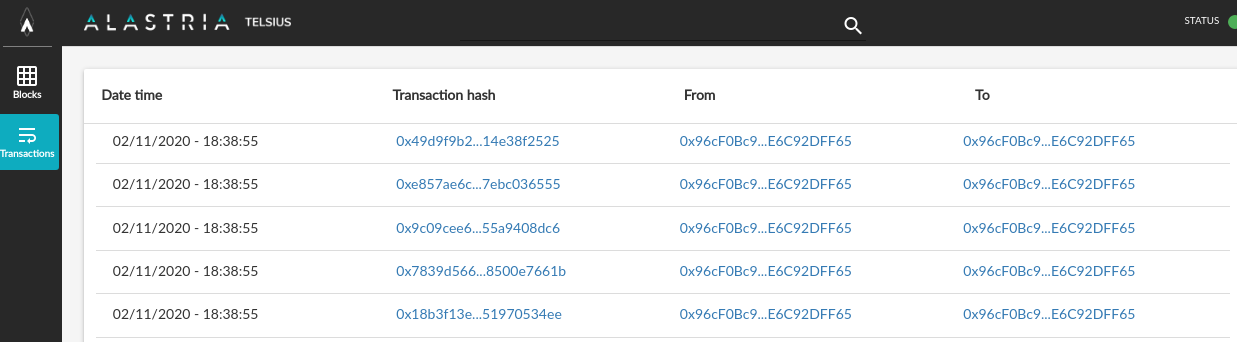
\includegraphics[width=1.1\textwidth]{Alastria-block-exporer.png}
                \caption{Alastria's Block explorer}
                \label{fig:alastria_block_explorer}
            \end{figure}
            \item \textbf{Immutability}. This property ensures that once something has been entered into the blockchain, it cannot be tampered or modified.
        \end{itemize}
        
        \subsubsection{How does Blockchain work?}
            A Blockchain is a growing list of records, called blocks (figure \ref{fig:linked_blocks}), that are linked using cryptography. Each block contains a hash of the previous block, the timestamp and a batch of valid transaction hashes encoded into a Merkle tree. The linked blocks form a chain. This iterative process confirms the integrity of the previous block, all the way back to the original genesis block (the first block of the network).
            \begin{figure}[h]
                \centering
                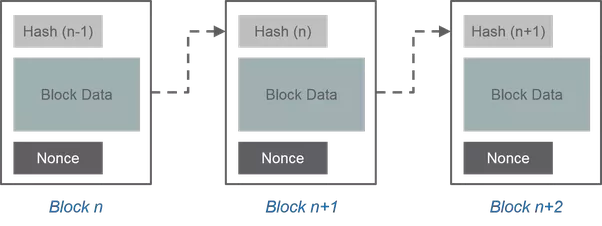
\includegraphics[width=1.0\textwidth]{block-example.png}
                \caption{Visual example of linked blocks}
                \label{fig:linked_blocks}
            \end{figure}
            
        \subsubsection{Types of blockchains}
            There are different kinds of Blockchain networks, each one with different features (figure  \ref{fig:blockchain_classification}). One of the most common classification is according to the architecture. The following figure shows a table with the classification.
            \begin{figure}[h]
                \centering
                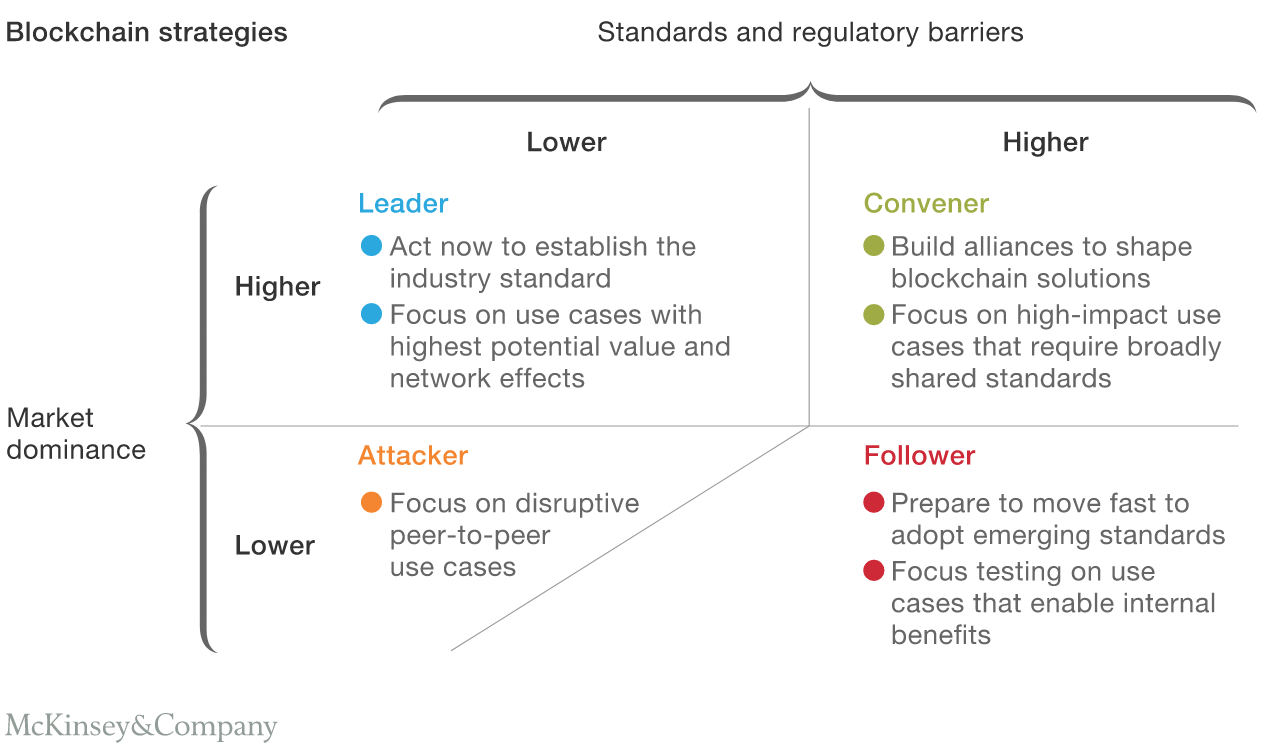
\includegraphics[width=1.0\textwidth]{Blockchain-types.png}
                \caption{Blockchain architecture classification by \textit{McKinsey\&Company}}
                \label{fig:blockchain_classification}
            \end{figure}

            \begin{itemize}
                \item \textbf{Public}. A public network is the one where everyone can join. Some examples of public networks are Bitcoin, Ethereum and Litecoin.
                \item \textbf{Private}. A private network is the one where only authorized members can join. Some examples of private networks are Quorum and Monax.
                \item \textbf{Permissionless}. A permissionless network is a private or public blockchain where every member can read and write.
                \item \textbf{Permissioned}. A permissioned network is a private or public blockchain where every member can read but only some can write. Some examples of public permissioned networks are Alastria and LACChain.
            \end{itemize}          
            Also, there are two more types of blockchain networks on the rise.
            \begin{itemize}
                \item \textbf{Consortium} or \textbf{hybrid networks}. These networks are private and permissioned, operated by known entities such as stakeholders of a given industry regrouped in a consortium or exploiting a shared platform. Some known examples are \textit{Hyperledger} \textit{Fabric}, \textit{R3 Corda} and \textit{Multichain}.
                \item \textbf{Blockchain as a Service} (BaaS). These are cloud platforms hosted by a service provider to deploy blockchain applications. The service provider manages the blockchain network while the customer defines the business logic. Some of the examples are \textit{Amazon (AWS)} and \textit{Oracle} blockchain platforms.
            \end{itemize}
            
            \subsubsection{Uses of blockchain}
                With the different properties of blockchain technology, and the different types of networks, there are a lot of use cases (figure \ref{fig:blockchain_uses}). The best known use case is using the blockchain as a payment infrastructure, the best example is Bitcoin. But there are a lot of other use cases shown in the next figure.\\
                \begin{figure}[h]
                    \centering
                    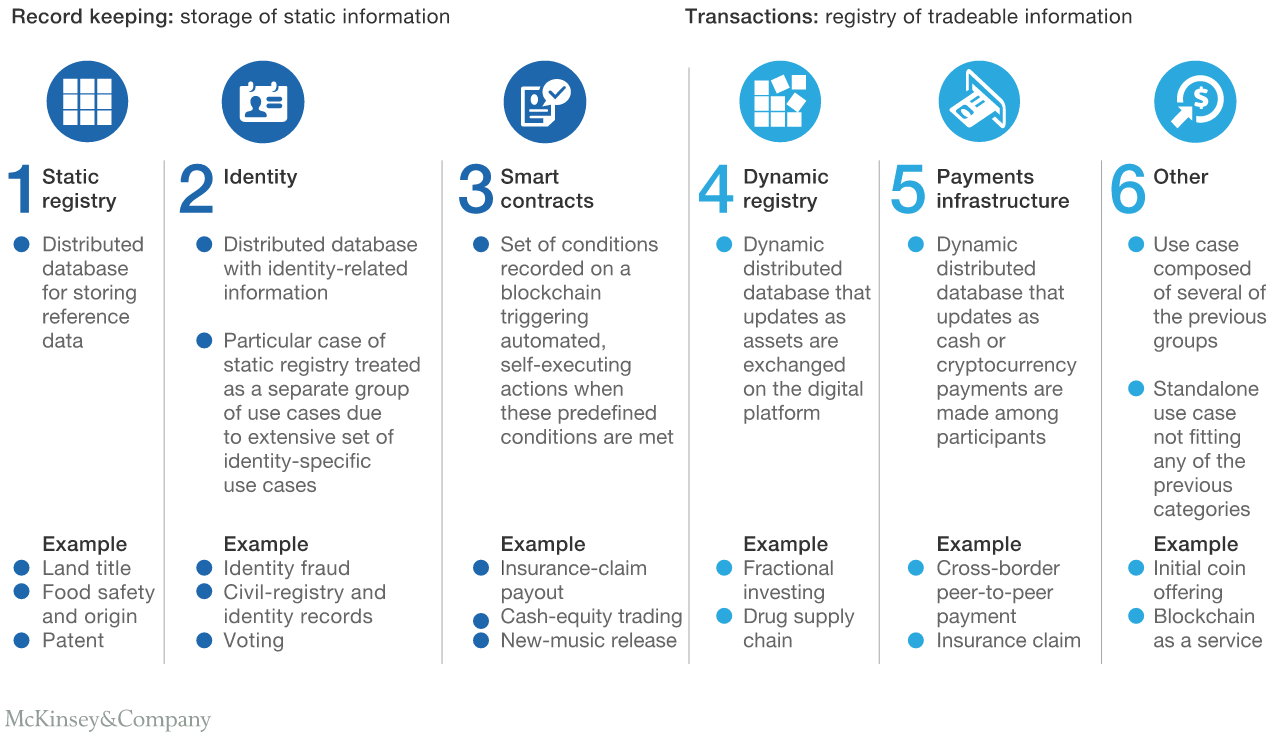
\includegraphics[width=0.95\textwidth]{Blockchain-uses.png}
                    \caption{Blockchain use cases table by \textit{McKinsey\&Company}}
                    \label{fig:blockchain_uses}
                \end{figure}
                
                In this document we are going to focus on the \acrfull{ssi} using blockchain.

    \subsection{Ethereum}
        Ethereum\cite{ethereum} (figure \ref{fig:ethereum_logo}) is an open-source, public, blockchain-based distributed ledger featuring smart contract functionality. It enables developers to build blockchain applications with business logic that execute in a trustless environment, while leveraging the high availability of the Ethereum network. 
        \begin{figure}[h]
            \centering
            
\includegraphics[width=0.5\textwidth]{ethereum-logo-portrait-purple.png}
            \caption{Ethereum logo}
            \label{fig:ethereum_logo}
        \end{figure}
        The principles behind Ethereum philosophy are\cite{ethereumWhitepaper}:
        \begin{itemize}
            \item \textbf{Simplicity}. The Ethereum protocol should be as simple as possible.
            \item \textbf{Universality}. Ethereum provides an internal Turing-complete scripting language. This language can be used to construct any logic, and any business case.
            \item \textbf{Modularity}. The Ethereum protocol is designed to be as modular as possible, to allow if one was to make a small protocol modification in one place, the application stack would continue to function as normally. 
            \item \textbf{Agility}. The protocol can be modified.
            \item \textbf{Non-discrimination} and \textbf{non-censorship}. The protocol should not restrict any usage.
        \end{itemize}
        
        \subsubsection{Ether}
            Ether (ETH) is the native cryptocurrency used on the Ethereum network and is used to compensate miners who secure transactions. It is used to pay for gas, a unit of computation used in transactions and other state transitions.
            Ether also has many current use cases, such as a store of value, a medium of exchange, and a unit of account.
            
        \subsubsection{Ethereum Accounts}
            An Ethereum account or simply an “account” is the combination of an Ethereum address and it’s private key. An account can hold balance (Ether) and can send transactions. In Ethereum there are 2 types of accounts.
            \begin{itemize}
                \item \textbf{Externally owned accounts} (EOA). These accounts are a combination of public address and private key. This accounts:
                \begin{itemize}
                    \item Has an ether balance
                    \item Can send transactions to Smart Contracts
                    \item Can send and receive ether to/from another account
                    \item Is controlled by private keys
                    \item Has no associated code
                \end{itemize}
                \item \textbf{Contract accounts}: These accounts don’t have a corresponding private key. These accounts are generated when a Smart Contract is deployed in the blockchain. They are normally called “contracts” instead of contract accounts. A contract:
                \begin{itemize}
                    \item Has an ether balance
                    \item They can receive ether just like EOA
                    \item Has associated code
                    \item Code execution is triggered by transactions or calls received from other contracts or accounts
                    \item When executed can manipulate its own persistent storage
                \end{itemize}
            \end{itemize}
        
        \subsubsection{Ethereum wallet}
            Wallets are software that are used to store and manage Ethereum accounts. Wallets allow the user to manage multiple accounts, provide functionality to sign transactions, track balances and so on. Wallets can be classified into two types.
            \begin{itemize}
                \item \textbf{Non-deterministic} wallet. These wallets use a random private key and generate a private key from it.
                \item \textbf{Deterministic} wallet. In this wallet, keys are derived from a seed. The seed allows a user to easily back up and restore a wallet without needing any other information, and in some cases allow the creation of public addresses without the knowledge of the private key.
            \end{itemize}
        
        \subsubsection{Ethereum stack}
            Like any software stack, the complete "Ethereum stack"\cite{ethereumStack} will vary from project to project depending on your business goals. However, the typical layers are:
            \paragraph{Ethereum Virtual Machine (EVM)}
                The Ethereum Virtual Machine\cite{evm}, normally known as EVM is a software designed to emulate a machine with certain capabilities that make the Ethereum blockchain possible. We can program instructions for the EVM, using a series of opcodes, which we can then compile and translate into a specific bytecode or language that the EVM can understand and execute.\\
                
                The opcodes perform standard stack operations like \textit{XORAND}, \textit{ADD}, \textit{SUB}, etc. The EVM also implements a number of blockchain-specific stack operations, such as \textit{ADDRESS}, \textit{BALANCE}, \textit{SHA3}, \textit{BLOCKHASH}, etc. More specific information can be found at the official documentation\cite{opcodes}.\\
                
                To make programming easier for the virtual machine, a specialized high-level language called Solidity was created. This programming language is used to create Smart Contracts. Solidity first transforms opcodes and then these to bytecode. This bytecode is finally executed by the EVM to perform the specified operations of a  Smart Contract. All this means that the EVM can function as a real computer, executing from the simplest to the most complex operations.\\
                
                In the following sections we will talk in detail about the Smart Contracts and Solidity.
                
            \paragraph{EVM Characteristics}
                The EVM has a series of unique characteristics\cite{ethereumGavin}\cite{ethereumDocu}:
                \begin{itemize}
                    \item It provides a \textbf{high level of security}. As it is a virtual machine limited in the instructions (opcodes) and the way they are executed, EVM is capable of executing unreliable codes without disastrous consequences.
                    \item The EVM is a \textbf{completely decentralized} build. Each node within the Ethereum network runs a copy of the virtual machine and is synchronized with the rest of the nodes that make up the network. This guarantees that the instructions given by the EVM are executed as long as there is at least one active node. This allows access to the system from anywhere in the world, resisting censorship and guaranteeing access to network resources. Furthermore, it does not require the participation of third parties, and resources can’t be modified or altered.
                    \item Applications can be executed on the same blockchain network, without affecting other operations.
                    \item EVM is able to follow the “rules” of Smart Contracts.
                    \item The EVM has the ability to execute a series of well-defined opcodes.
                \end{itemize}
                
            \paragraph{How does it work?}
                The figure \ref{fig:blockchain_stack} defines how the EVM works\cite{queEsEvm}.
                \begin{figure}[h]
                    \centering
                    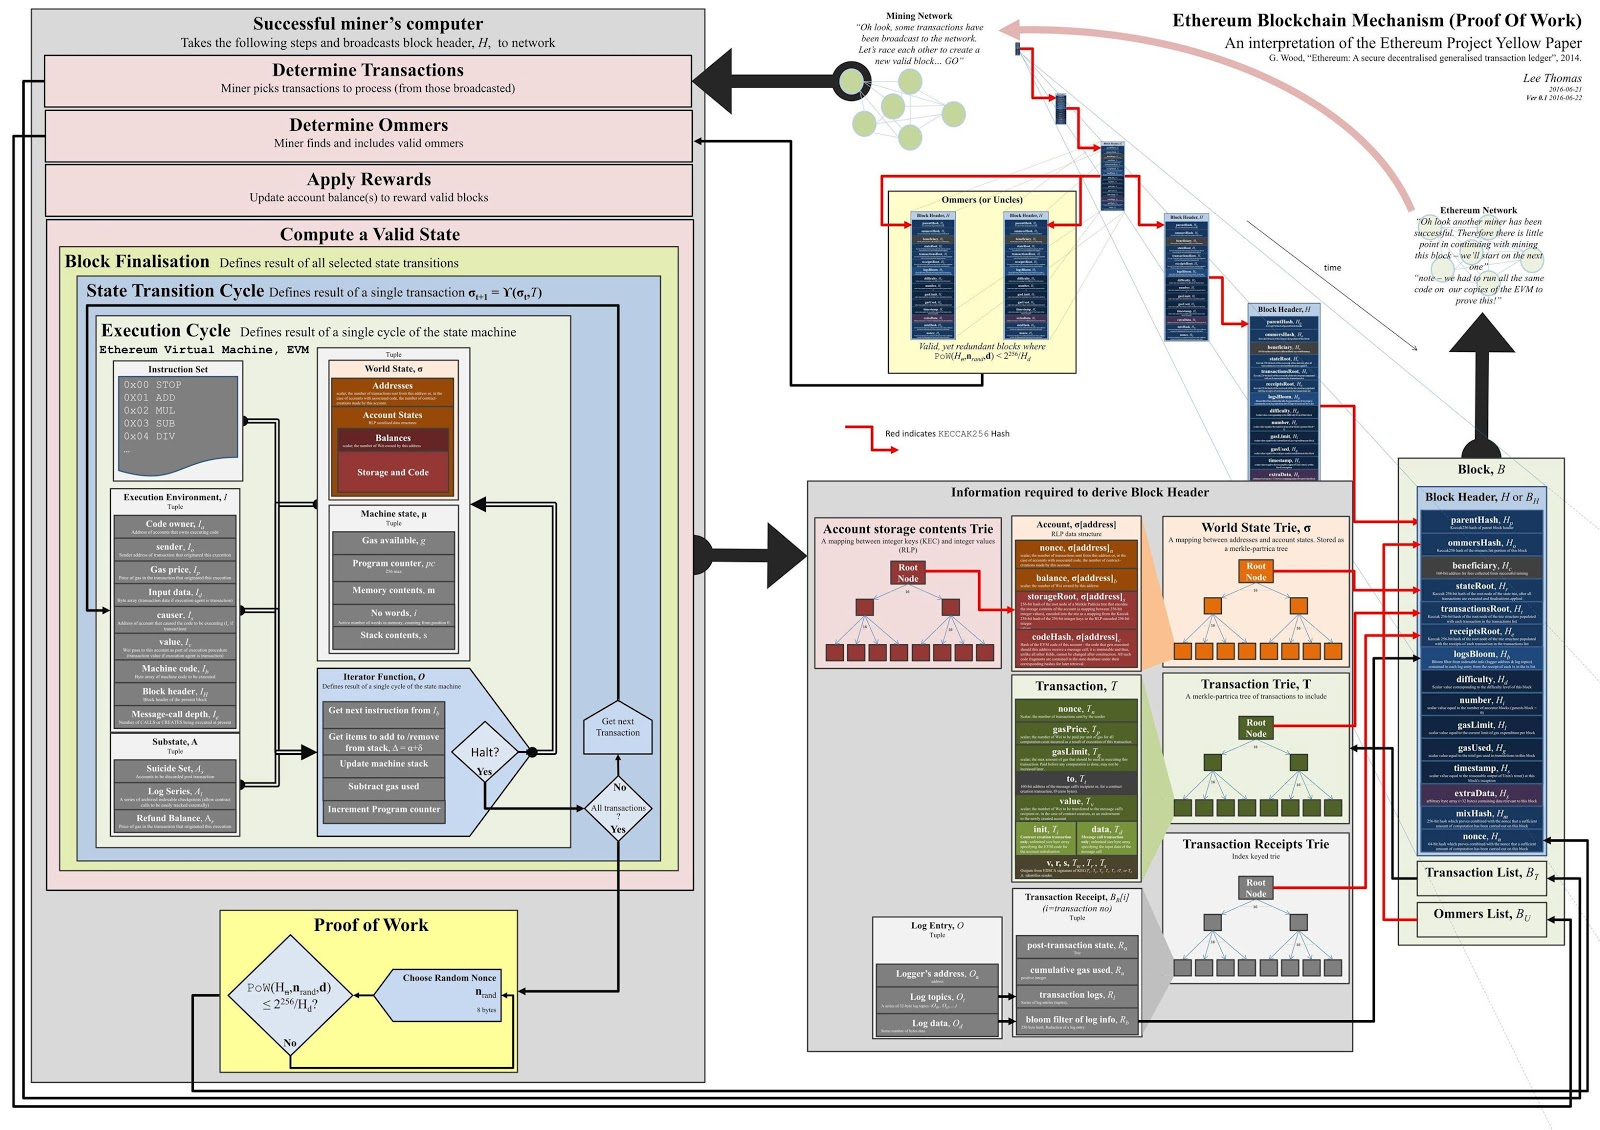
\includegraphics[width=1\textwidth]{evm-stack.jpeg}
                    \caption{EVM stack schema}
                    \label{fig:blockchain_stack}
                \end{figure}

                The Smart Contracts made with Solidity are compiled and converted to opcodes. These opcodes are transformed to bytecode, so it does facilitate the performance of the EVM tasks.\\

                Thus, each transaction and operation that is carried out on the Ethereum blockchain goes through this process, and its execution is carried out by the EVM, which at the end records everything on the Ethereum blockchain, leaving a public record of those operations. 

        \subsubsection{Smart Contracts}
            Sam Richards\cite{smartContracts}, a Software Engineer working on Ethereum defines the Smart Contract as 
            \begin{quote}
                \textit{a snippet of code that runs on the Ethereum blockchain. It's a collection of functions and data that resides at a specific address on the Ethereum blockchain.}

                \textit{Smart contracts are a type of Ethereum account. This means they have a balance and they can send transactions over the network. However they're not controlled by a user, instead they are deployed to the network and run as programmed. User accounts can then interact with a smart contract by submitting transactions that execute a function defined on the smart contract. Smart contracts can define rules, like a regular contract, and automatically enforce them via the code.}
            \end{quote}

        \subsubsection{Solidity}
            \begin{figure}[h]
                \centering
                
\includegraphics[width=0.4\textwidth]{solidity-logo.jpg}
                \caption{Solidity logo}
                \label{fig:solidity_logo}
            \end{figure}
            
            Solidity (figure \ref{fig:solidity_logo}) defines itself as an object-oriented, high-level language for implementing Smart Contracts. Smart Contracts are programs which govern the behaviour of accounts within the Ethereum state.\\
            
            Solidity\cite{solidityGit} was influenced by \textit{C++}, \textit{Python} and \textit{JavaScript} and is designed to target the Ethereum Virtual Machine (EVM). Solidity is statically typed, supports inheritance, libraries and complex user-defined types among other features.\\

            Below is an example\footnote{Source code from AlastriaIdentityIssuer.sol\cite{AlastriaIdentityIssuer}}
 of a Smart Contract written in Solidity\footnote{More details about Solidity can be found in the official documentation\cite{solidity}} (listing  \ref{lst:AlastriaIdentityIssuer}).
            
            \lstinputlisting[label={lst:AlastriaIdentityIssuer}, caption=Source code from AlastriaIdentityIssuer.sol, language=Solidity]{examples/SmartContracts/AlastriaIdentityIssuer.sol}

        \subsubsection{Ethereum Nodes}
            A Node refers to a piece of software which is an implementation of Ethereum that verifies all transactions in each block, keeping the network secure and the data accurate. They collectively store the state of the Ethereum blockchain and reach consensus on transactions to mutate the blockchain state.\\
            
            There are three types of nodes.
            \begin{itemize}
                \item \textbf{Full node}. These types of nodes store full blockchain data, participate in block validation, verifies all blocks and states and serves the network and provides data on request. Also, all states can be derived from a full node.
                \item \textbf{Light node}. Stores the header chain and requests everything else. Can verify the validity of the data against the state roots in the block headers and it is useful for low capacity devices, such as embedded devices or mobile phones, which can't afford to store gigabytes of blockchain data.
                \item \textbf{Archive node}. Stores everything kept in the full node and builds an archive of historical states. These nodes can be handy for services like block explorers, wallet vendors, and chain analytics.
            \end{itemize}
            By connecting your application to an Ethereum node via JSON RPC, your application is able to read data from the blockchain as well as broadcast new transactions to the network.

        \subsubsection{Ethereum Client APIs}
            While APIs are not a necessary piece of the stack, they abstract away much of the complexity of interacting directly with Ethereum nodes and Smart contracts.\\
            
            Most of these APIs are open source and maintained by the Ethereum community.

        \subsubsection{End User Applications}
            The final part of the stack is the user-facing applications, primarily web and mobile apps.  They are made for users so they do not need to know the application they're using is built using a blockchain. Also the end user applications are made to hide the complexity from the user.
            
        \subsubsection{Ethereum 2.0 (Eth2)}
            Eth2\cite{eth2} is a long-planned upgrade to the Ethereum network, it will reduce energy consumption, allow the network to process more transactions, and increase security.  Ethereum will become a proof-of-stake blockchain and introduce shard chains. Shard chains are like parallel blockchains that sit within Ethereum and take on a portion of the network's processing work.\\
            
            The phase 1 of Ethereum 2.0 is supposed to happen in 2021. The roadmap can be checked in the official website\cite{eth2Roadmap}.
            

    \subsection{JSON-RPC}
        JSON-RPC is a remote procedure call protocol (RPC) encoded in JSON. It is a simple protocol that defines only a few data types and commands. JSON-RPC allows for notifications (data sent to the server that does not require a response) and for multiple asynchronous calls. It uses JSON \textit{RFC-4627}\cite{rfc4627} as data format.\\
        
        The first officially released specification was \textit{JSON-RPC 1.0}\cite{json-rpc-1} published in 2005, but the last official specification is \textit{JSON-RPC 2.0}\cite{json-rpc-2} published in 2010 with several improvements.
        
        \subsubsection{JSON}
            JavaScript Object Notation mostly known as JSON is a lightweight data-interchange format. It is human readable and easy to write. Also, it is easy for machines to parse and generate. It is based on a subset of the JavaScript Programming Language Standard ECMA-262 3rd Edition - December 1999. JSON is a text format that is completely language independent but uses conventions that are familiar to several languages such as \textit{C}, \textit{C++}, \textit{Java}, \textit{JavaScript}, \textit{Perl}, \textit{Python} and many others.\\
                        
            JSON is built on two structures\cite{jsonSchema}:
            \begin{itemize}
                \item A collection of name-value pairs (figure \ref{fig:json_objects}). In various languages, this is realized as an Object, Record, Struct, Dictionary, ...
                \begin{figure}[h]
                    \centering
                    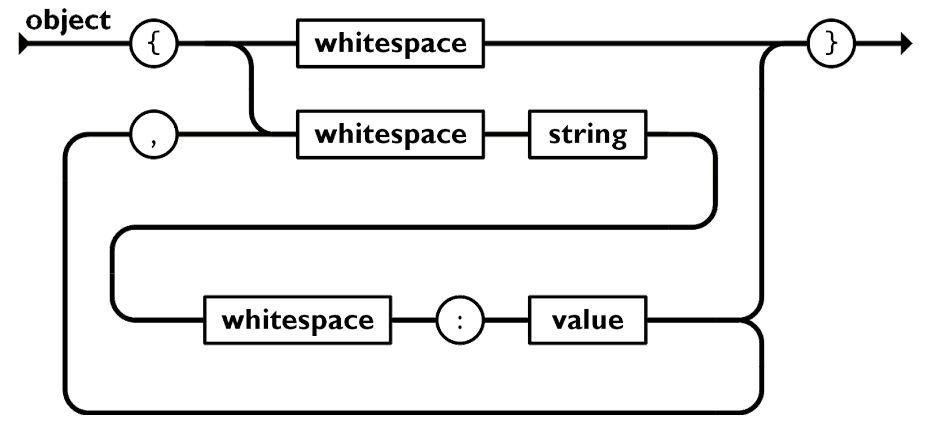
\includegraphics[width=0.6\textwidth]{json-objects.png}
                    \caption{JSON objects schema}
                    \label{fig:json_objects}
                \end{figure}
                \item An ordered list of values (figure \ref{fig:json_arrays}). In most languages, this is realized as an Array, Vector, List, ...
                \begin{figure}[h]
                    \centering
                    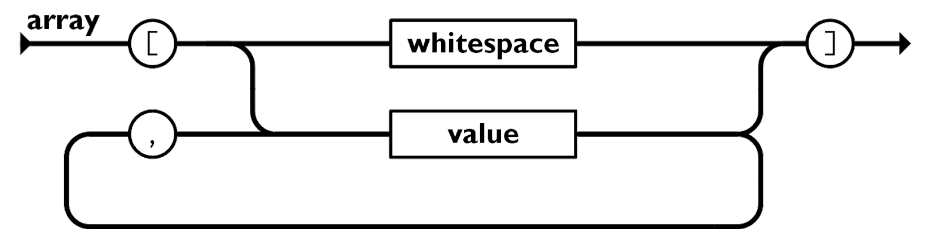
\includegraphics[width=0.6\textwidth]{json-arrays.png}
                    \caption{JSON array schema}
                    \label{fig:json_arrays}
                \end{figure}
            \end{itemize}

        \subsubsection{RPC}
            A remote procedure call (RPC)\cite{rpc} is when a computer program causes a procedure to execute in a different address space (commonly on another computer), which is coded as if it were a local procedure call. That is, the programmer writes essentially the same code whether the program will run locally or in a remote machine.\\
            
            The transparency is one of the great strengths of RPC, because the application software does not contain any communication code, it is independent of:
            \begin{itemize}
                \item The communication hardware and protocols used
                \item The operative system
                \item The calling sequence needed to use the communication software layer
            \end{itemize}
            
            \paragraph{How RPC works}
                From the point of view of a remote call, the calling program is known as client, and the subroutine it calls is known as the server\cite{rpcInOS}\cite{howRPC}. When the client calls the server, the RPC system must take care of:
                \begin{itemize}
                    \item Taking all the parameters which are passed to the subroutine and transferring them to the remote node
                    \item Having the subroutine executed on the remote node
                    \item Transferring back all the parameters which are returned to the calling routine
                \end{itemize}
                
                In the next figure (figure \ref{fig:rpc_schema}) we can see the typical RPC communication schema.
                \begin{figure}[h]
                    \centering
                    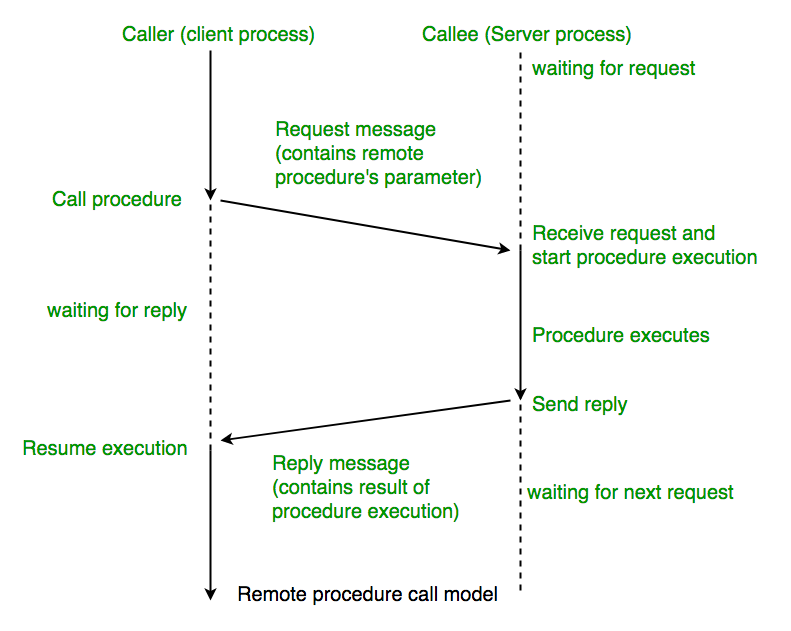
\includegraphics[width=0.7\textwidth]{rpc.png}
                    \caption{RPC schema}
                    \label{fig:rpc_schema}
                \end{figure}
                The most common method of doing this is by the use of stub modules (figure \ref{fig:rpc_mechanism}). The client is linked to a client stub module. This is a subroutine which looks like the remote subroutine, but on the inside, it is almost empty. All it does is take the values of the parameters which are passed to it, and put them in a message. This is known as marshalling.\\

                The client stub then uses a routine in the RPC Run-Time System (RTS) to send the message off and wait for a reply message. When the reply arrives, the stub unmarshals the parameters that were returned in the reply message, putting their values into the variables of the calling program. The client stub then returns to the calling program just like a normal subroutine.\\

                The server stub (located in the remote machine) is called by the RPC RTS when the message arrives from the client. The server stub performs the unmarshall of the parameters passed to the subroutine, calling the subroutine, and marshalling the return parameters. 
                \begin{figure}[h]
                    \centering
                    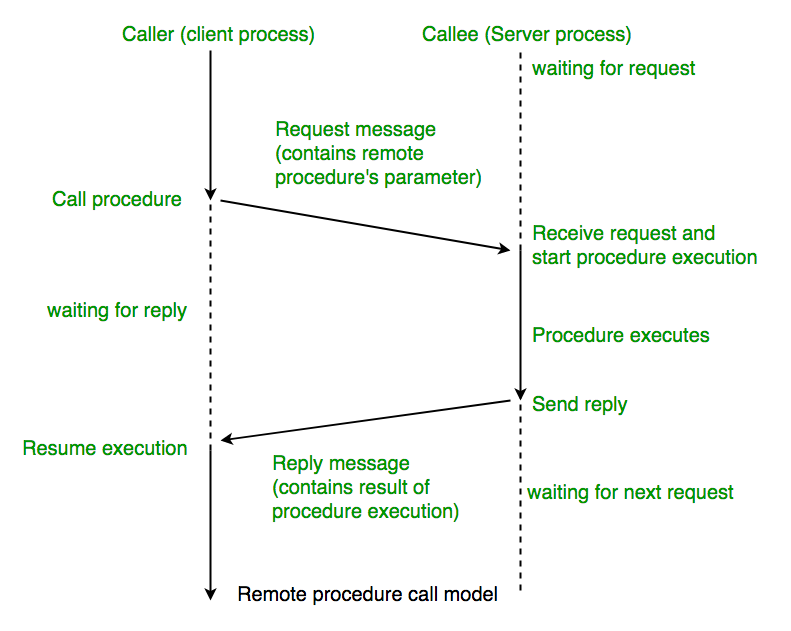
\includegraphics[width=0.7\textwidth]{rpc-mecha.png}
                    \caption{RPC mechanism}
                    \label{fig:rpc_mechanism}
                \end{figure}
                All the communication details are handled by the RPC RTS, so the stubs contain only the code which is specific to the application involved\cite{rpc2}.
                \begin{itemize}
                    \item In order to produce stub modules, it is need to know
                    \item The names of the procedures in the package (set of procedures)
                    \item The number of parameters which they take
                    \item The data type of each parameter
                    \item The direction in which each parameter is transferred
                \end{itemize}
        \subsubsection{JSON-RPC 1.0}
            The general mechanism consists of two peers establishing a data connection\cite{json-rpc-1}. Peers may invoke methods provided by the older peer. To invoke a remote method, a request serialized using JSON is sent. The request is a single JSON Object with three properties: 
            \begin{itemize}
                \item \textbf{method}: The name of the invoked method.
                \item \textbf{params}: The params passed as arguments to the method. It is an Array of Objects.
                \item \textbf{id}: The request id. It can be of any type. It is used to match the response with the reply. If it is a notification request, it must be Null.
            \end{itemize}
            The request must be replied unless it is a notification (does not need a response). The response is also a single Object serialized using JSON and has this properties:
            \begin{itemize}
                \item \textbf{result}: The Object returned by the invoked method. It is Null in case there was an error.
                \item \textbf{error}: An error Object if there was an error while invoking the method. It is Null if there was no error.
                \item \textbf{id}: The id of the request that was sent. 
            \end{itemize}
            JSON-RPC does not require a certain transport protocol, but TCP/IP socket streams are encouraged. The request and the response are sent to the peers through byte streams.\\

            Also HTTP can be used as the communication transport. The request must be sent as an \textit{HTTP POST} with all the serialized Objects. Once the client has received the response, it must reply with another \textit{HTTP POST}. A non-valid request will result in closing the connection.
        \subsubsection{JSON-RPC 2.0}
            This specification\cite{json-rpc-2} works almost the same way as the JSON-RPC 1.0 but it has several upgrades.\\
            
            The request Object has the following properties:
            \begin{itemize}
                \item \textbf{jsonrpc}: The version of the JSON-RPC protocol. It must be exactly “2.0”.
                \item \textbf{method}: A String containing the name of the method.
                \item \textbf{params}: A Structured value (Object or Array) with the parameter values passed as arguments to the method.
                \item \textbf{id}: It is a String, Number or \textit{Null} identifier. If it is not included, it is assumed to be a notification. Normally it should not be \textit{Null} because this specification uses a value of \textit{Null} for responses with unknown id. Also, JSON-RPC 1.0 uses \textit{Null} for notifications, and it causes confusion in handling.
            \end{itemize}
            Similarly, the response from the server is expressed as a single JSON Object with the following properties:
            \begin{itemize}
                \item \textbf{jsonrpc}: As in the request, it must exactly be “2.0”
                \item \textbf{result}: It is required on success, but must not exist if there was an error.
                \item \textbf{error}: It is required on error, but must not exist if there was no error. It must be an Object with the following properties:
                \begin{itemize}
                    \item \textbf{code}: A Number that indicates the error type occurred.
                    \item \textbf{message}: The provided short description of the error.
                    \item \textbf{data}: A Primitive (String, Number, Boolean or Null) or Structured (Object or Array) with additional information about the error. This may be omitted and it is defined by the server. The error codes are nearly the same as those suggested for XML-RPC\cite{rpc-err}.
                \end{itemize}
                \item \textbf{id}: This property must be the same as the value of the requested Object. If there was an error, it must be \textit{Null}.
            \end{itemize}
            To send several requests at the same time, the client may send an Array with all the request objects. It is called batch. The response from the server should be another Array containing the response objects after all the requests have been processed. The server may process the batch as a set of concurrent tasks. Also, the response objects may be returned in any order within the Array. Thanks to the id server and client will match the context between requests and responses.
            
        \subsection{JSON Web Tokens}
            In the RFC-7519\cite{rcf-jwt}, the \acrfull{jwt} is defined as:
            \begin{quote}
                \textit{\acrfull{jwt} is a compact claims representation format intended for space constrained environments such as HTTP Authorization headers and URI query parameters.  \acrfull{jwts} encode claims to be transmitted as a JSON object that is used as the payload of a \acrfull{jws} structure or as the plaintext of a \acrfull{jwe} structure, enabling the claims to be digitally signed or integrity protected with a \acrfull{mac} and/or encrypted. \acrshort{jwts} are always represented using the \acrshort{jws} Compact Serialization or the \acrshort{jwe} Compact Serialization.} 
           \end{quote}
          
          Basically a \acrshort{jwt} is a JSON that has three parts:
          \begin{itemize}
              \item \textbf{Header}: provides important information about the token.
              \item \textbf{Payload}: it contains the actual information that will be transmitted to the application. The information is provided as key-value pairs. The keys are called claims.
              \item \textbf{Signature}: It is created using the Base64 encoding of the header and payload, as well as the specified signing or encryption method. The structure is defined by \acrfull{jws}.
          \end{itemize}
          Below (figure \ref{fig:jwt-ex}) we can see an example of signed and unsigned \acrshort{jwt}.
          \begin{figure}[h]
                \centering
                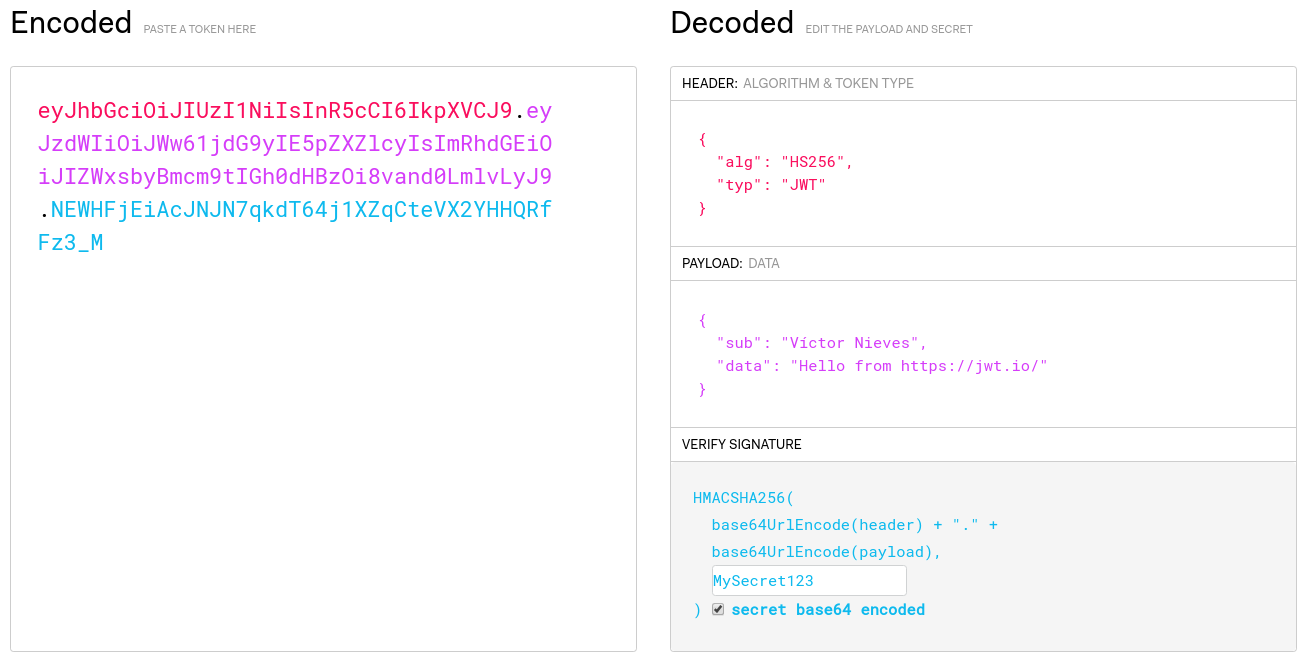
\includegraphics[width=1\textwidth]{jwt-example.png}
                \caption{Example of signed and unsigned \acrshort{jwt}}
                \label{fig:jwt-ex}
          \end{figure}

        
        \subsection{Self-Sovereign Identity}
            The idea of the \acrlong{ssi} was born to solve the problems with the current physical and digital identifications.\\
            Some of the physical IDs problems are:
            \begin{itemize}
                \item The process of obtaining them is time consuming, bureaucratic and costly. For both the ID Owner and Issuer Organization. 
                \item If you lose your ID and need to obtain a new one.
                \item Physical IDs can be defrauded with impersonation and ID theft. The only way to check its authenticity is often by contacting the issuing organization.
                \item They are not private.
            \end{itemize}
            Also, some problems with the current digital IDs are:
            \begin{itemize}
                \item Having to register and sign up with different login credentials to every new online service is uncomfortable for the user. 
                \item Tedious on-boardings.
                \item Managing multiple passwords is hard and using the same password is a security risk.
                \item The user has no control over what data is being shared and with whom.
                \item The verification of your credentials is dependent on the availability of the issuer.
                \item Third party login services have a financial incentive to collect and store your data.
                \item The user's personal data is stored on the issuer’s servers. Centralized storages of personal data create \textit{“honeypots”}. This data is at risk of breaches, leaks or hacks.
            \end{itemize}

            \acrfull{ssi} is a digital identification scheme in which the user acquires the responsibility of managing how and in what quantity their personal data is used. To do this, it allows the creation of digital \textit{“identity cards}” that can be general for any service or specific for each case. \\
            The main characteristics of \acrlong{ssi} are\cite{ssi-guide}:
            \begin{itemize}
                \item It is secure and digital peer-to-peer channel is established between Issuer, owner and Verifier.
                \item When credentials are exchanged not even the \acrlong{ssi} system provider knows what is being exchanged.
                \item Credentials are tamper-proof through the use of cryptography.
                \item They are private and under the owner control. \acrshort{ssi} uses Selective Identity disclosure technology.
                \item The Owner chooses what data they want to “show” and is always in control of the relationship with ID Verifiers.
                \item Credentials can be verified anywhere, at any time.
                \item Personal Data is not stored on centralized servers.
                \item \acrshort{ssi} tries to abolish multiple passwords. You just need to know your wallet password.
            \end{itemize}

            \subsubsection{How does it work?}
                In order to explain how the \acrshort{ssi} works, we have to see some concepts previously.
                \paragraph{Actors}
                    The figure \ref{fig:trust-triangle} explains the different actors\cite{ssi-guide} that take place in the process.
                    \begin{figure}[h]
                        \centering
                        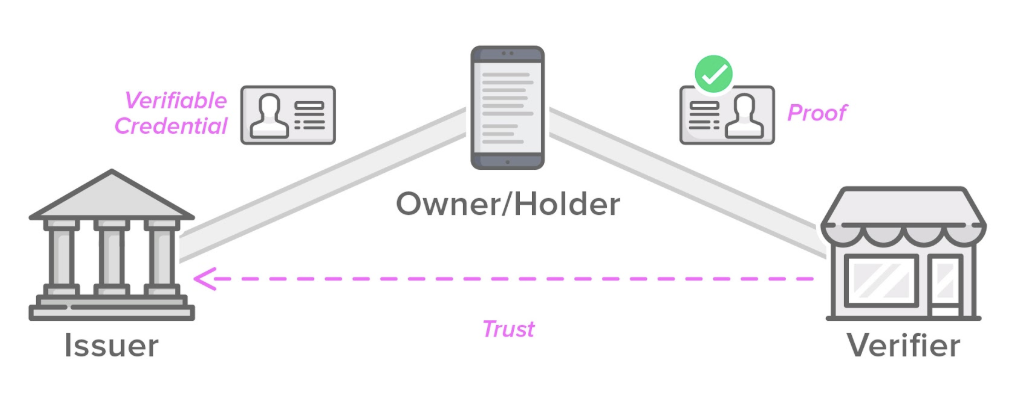
\includegraphics[width=0.7\textwidth]{trust-triangle.png}
                        \caption{Trust triangle / Actors in \acrshort{ssi}}
                        \label{fig:trust-triangle}
                    \end{figure}
                    \begin{itemize}
                        \item \textbf{Owner / Holder}: orders the creation of credentials. He stores the credentials locally. He has the power to revoke access to these credentials.
                        \item \textbf{Issuer}: provides a digital service. It needs to identify users. Does not need to store user data.
                        \item \textbf{Verifier}: creates the credentials with the data provided by the user. It does not store user data (although it has access to it at the time of creation of the credential).
                    \end{itemize}
            
                \paragraph{Verifiable Credentials}
                    According to the World Wide Web Consortium \textit{(W3C)}\cite{w3c-vc}\footnote{\label{footnote-w3c}More information about Verifiable Credentials and Verifiable Presentations can be found in the main web page of W3C\cite{w3c-vc}}:
                    \begin{quote}
                        \textit{A verifiable credential can represent all of the same information that a physical credential represents. The addition of technologies, such as digital signatures, makes verifiable credentials more tamper-evident and more trustworthy than their physical counterparts.}
                    \end{quote}
                    In the figure \ref{fig:ssi-vc}, we can see clearly the relationship between Issuer, Holder and Verifier and how a Verifiable Data Registry (normally a blockchain) is used to verify the credentials’ data without the need to contact the issuing party.
                    \begin{figure}[h]
                        \centering
                        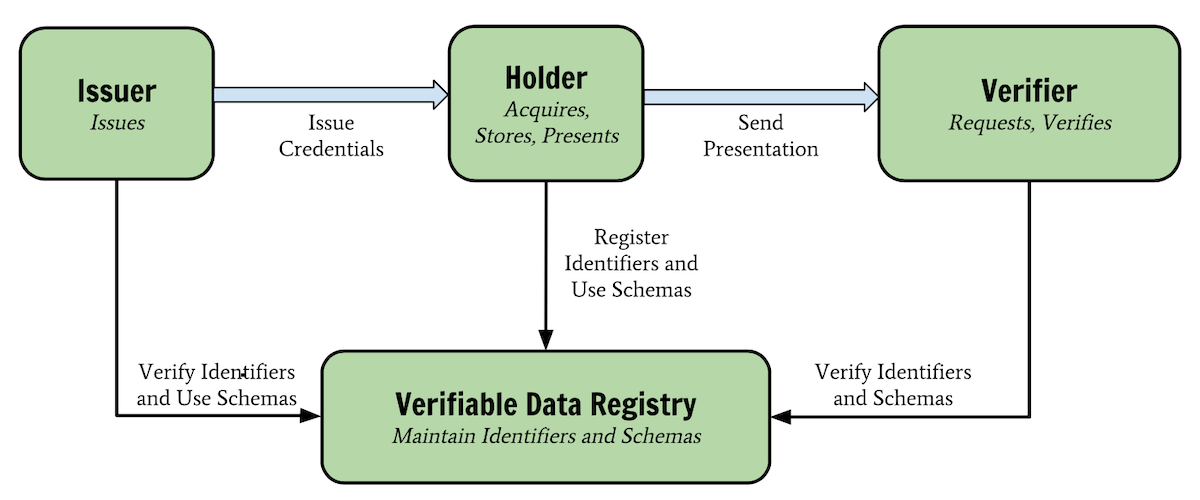
\includegraphics[width=1.0\textwidth]{ssi-vc.png}
                        \caption{The roles and information in a \acrshort{ssi} ecosystem by W3C}
                        \label{fig:ssi-vc}
                    \end{figure}
                
                \paragraph{Verifiable Presentations}
                    According to W3C\cite{w3c-vc}\footref{footnote-w3c}:
                    \begin{quote}
                        \textit{A verifiable presentation expresses data from one or more verifiable credentials, and is packaged in such a way that the authorship of the data is verifiable. If verifiable credentials are presented directly, they become verifiable presentations. Data formats derived from verifiable credentials that are cryptographically verifiable, but do not of themselves contain verifiable credentials, might also be verifiable presentations.}
                        
                        \textit{The data in a presentation is often about the same subject, but might have been issued by multiple issuers. The aggregation of this information typically expresses an aspect of a person, organization, or entity.}
                    \end{quote}
                    In the figure \ref{fig:ssi-vp} we can see the components of a verifiable presentation.
                    \begin{figure}[ht] 
                        \centering
                        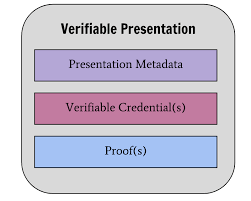
\includegraphics[width=0.5\textwidth]{ssi-vp.png}
                        \caption{Basic components of a verifiable presentation by W3C}
                        \label{fig:ssi-vp}
                    \end{figure}
                %\newpage % TODO: que no corte el texto de DIDs
                \paragraph{Decentralized Identifiers (DIDs)}
                    According to W3C\cite{w3c-did}\footnote{More information about the DIDs can be found in the main web page of W3C\cite{w3c-did}}:
                    \begin{quote}
                        \textit{Decentralized identifiers (DIDs) are a new type of identifier that enables verifiable, decentralized digital identity. A DID identifies any subject (e.g., a person, organization, thing, data model, abstract entity, etc.) that the controller of the DID decides that it identifies. In contrast to typical, federated identifiers, DIDs have been designed so that they may be decoupled from centralized registries, identity providers, and certificate authorities. Specifically, while other parties might be used to help enable the discovery of information related to a DID, the design enables the controller of a DID to prove control over it without requiring permission from any other party. DIDs are URIs that associate a DID subject with a DID document allowing trustable interactions associated with that subject.}
                        
                        \textit{Each DID document can express cryptographic material, verification methods, or service endpoints, which provide a set of mechanisms enabling a DID controller to prove control of the DID. Service endpoints enable trusted interactions associated with the DID subject. A DID document might contain the DID subject itself, if the DID subject is an information resource such as a data model.}
                    \end{quote}
                    
                \paragraph{Wallets}
                    A wallet\cite{ssi-wallets} is a private repository that allows its owner to store, manage, and present keys and identity credentials.\\
                    
                    Some of the properties every wallet should have are:
                    \begin{itemize}
                        \item Provide secure access to the owner.
                        \item Guarantee that only authorized entities can access to it.
                        \item Ensure security and data encryption.
                        \item Provide recovery for keys and credentials.
                        \item Be connected to the blockchain where the DID was registered.
                        \item Provide mechanism for subjects and issuers to change the status of their credentials.
                        \item Provide mechanism for the owner to erase all the data associated with them.
                    \end{itemize}
                    Normally, when we talk about wallet, we think in mobile wallets (mobile applications), but a wallet can also be in a desktop, browser, hardware or the cloud.
                
                \paragraph{Functioning}
                    In the architecture\cite{how-to-ssi} we find a credential provider (\textit{issuer}) that is responsible for signing the data provided by the user by creating a certificate. Then, it will be signed by the user, attesting that the certificate generated by the issuer does not contain missing or altered information.\\
                    
                    Signatures by both the user and the issuer are performed using DIDs, which are traditional asymmetric keys. The public key of both is stored publicly on the blockchain. In this way, later on, the service provider (\textit{verifier}) that wants to identify the user will only have to verify that the signatures are correct and that, therefore, the credential has not been altered and contains the same information that the user provided to the identity provider.\\
                    
                    In the next figure (figure \ref{fig:ssi-scheme}) we can see a graphic scheme of the explained above.
                    \begin{figure}[h]
                        \centering
                        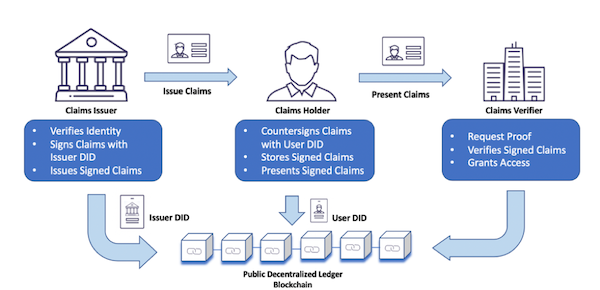
\includegraphics[width=1.0\textwidth]{how-to-ssi.png}
                        \caption{SSI functioning scheme}
                        \label{fig:ssi-scheme}
                    \end{figure}

            \subsubsection{Use cases}
                \acrlong{ssi} is benefiting several industries\cite{ssi-guide}, some examples are: streamlining bureaucratic procedures, improving a more efficient healthcare system, detecting academic and business fraud, creating a better user experience while onboardings or helping companies avoid personal data breaches and GDPR\cite{gdpr} fines.

            \subsubsection{Alastria}
                Alastria (figure \ref{fig:alastria_logo}) is the world’s first nation-wide, multi-sectorial, enterprise grade, permissioned blockchain network. A non-profit association open to all types of companies and organizations with the mission to contribute to the creation of a diverse innovation ecosystem. Alastria is technology agnostic and offers the networks promoted by its partners as well as a user centric Digital Identity model, the Alastria ID, focused on ensuring the legal validity of the transactions on the networks.
                \begin{figure}[h]
                    \centering
                    
\includegraphics[width=0.5\textwidth]{alastria-logo.png}
                    \caption{Alastria logo}
                    \label{fig:alastria_logo}
                \end{figure}
                \paragraph{Alastria ID}
                    Alastria ID (figure \ref{fig:alastria_id_logo}) is a digital identity model proposed by the Consortium for use in digital services, even beyond blockchain technology itself and inspired by the Self Sovereign Identity concept.\\
                    \begin{figure}[h]
                        \centering
                        
\includegraphics[width=0.2\textwidth]{alastria-id-logo.png}
                        \caption{Alastria ID logo}
                        \label{fig:alastria_id_logo}
                    \end{figure}
                
                    The Identity Commission of Alastria ID\cite{alastria-context} has taken a further step in the typical functionalities of this tool. It has followed the recommendations of the ID of the World Wide Web Consortium\cite{w3c} (W3C), the international community that develops Internet standards. It has even been improved. Alastria ID has been developed in accordance with the demanding European data protection regulations GDPR\cite{gdpr} (General Data Protection Regulation), and eIDAS\cite{eidas} (European system for the recognition of electronic identities).\\

                    The Alastria Standards Commission, which participates in all international and national standardization bodies, has collaborated in the process of the definition of the Alastria ID. The model specification inspired the Spanish identity standard UNE 71307\cite{une-71307} and the decentralized identity framework of EBSI\cite{ebsi} (European Blockchain Services Infrastructure), the blockchain of European public administrations.\\
                    
                    In the next section we will delve into the peculiarities and details of the different tools created by Alastria to facilitate the use of Alastria ID.

            \subsubsection{Other implementations}
                At present, \acrlong{ssi} is still at an early stage. However, there is already an extensive catalog of projects that show their potential. Different working groups and standardization agencies have been working to develop new standards and protocols that are the base of the \acrshort{ssi} model\cite{ssi-wallets}. Some of these groups are: the \textit{Decentralized Identity Foundation} (DIF), the \textit{European Blockchain Services Infrastructure} (EBSI), the \textit{Internet Engineering Task Force} (IETF), \textit{LACChain}, \textit{NIST}, \textit{Sovrin}, \textit{OASIS}, the \textit{OpenID Foundation} (OIDF), and the \textit{World Wide Web Consortium} (W3C).\\
                
                There are also a few existing solutions on the market which leverage new standards and protocols for \acrshort{ssi}:
                % TODO resumen de otras, como UPORT
                \paragraph{Serto/uPort}
                    Serto\cite{serto} (figure \ref{fig:uport}) formerly known as uPort\cite{uport} is a web-based wallet and identity management system created by ConsenSys\cite{consenSys}. This project allows users (people) to manage their own private and public keys, without the need for intermediaries. It allows these keys to be recovered without the user having to lose their identity. The system consists of a mobile application (wallet), where the user can manage their identity, can receive and issue claims. A claim is nothing more than a data structure where \textit{"someone says something about another person"}. These claims make up the identity of the user, and can be displayed to identify themselves in front of entities. The identity is controlled by the user, without problems of someone questioning the legitimacy or altering the identity data.
                    \begin{figure}[h]
                        \centering
                        
\includegraphics[width=.2\textwidth]{serto-logo.png}\hfill
                        
\includegraphics[width=.2\textwidth]{uport-logo.png}\hfill
                        
\includegraphics[width=.3\textwidth]{consensys-horizontal-logo.png}
                        \caption{Serto, uPort and ConsenSys logos}
                        \label{fig:uport}
                    \end{figure}
                    
                \paragraph{David19}
                    David19\cite{david19} (figure \ref{fig:david19}) emerges as a collaborative application in which any citizen can participate to promote digital transformation in order to face health emergencies caused by the COVID-19 pandemic in 2019. This project created by LACChain\cite{lacchain} allows users (citizens) to share their information in solidarity, in a secure and anonymous way through self-claimed credentials. With this information, risk maps can be generated in real time, thus allowing authorities to make key decisions in managing the pandemic.\\
                    \begin{figure}[h]
                        \centering
                        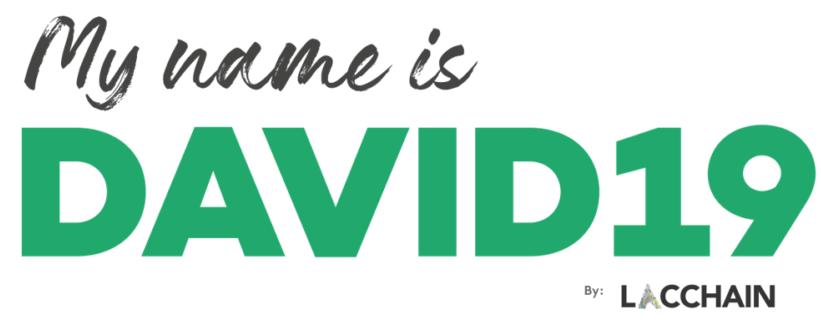
\includegraphics[width=.3\textwidth]{logo-david19.png}
                        \caption{David19 logo}
                        \label{fig:david19}
                    \end{figure}
                    
                    In a second phase\cite{que-es-david19}, it is proposed that the entities join the ecosystem, and that they can issue more sophisticated credentials, such as permits to return to work, medical certifications or academic degrees. The ultimate goal of David19 is for a person to only need a mobile device (wallet) to demonstrate that they are fit to get on a plane, return to work, visit a museum, etc., all in compliance with applicable regulations. The final objective of David19 is that a person only needs a mobile device (wallet) to demonstrate that they are healthy to get on a plane, return to work, visit a museum, etc., all in compliance with the regulations that apply at the time and the place.

                \paragraph{Hyperledger Indy}
                    Contributed by the Sovrin Foundation\cite{sovrin-yt}\cite{sovrin}, Hyperledger Indy\cite{indy-gh}\cite{indy} (figure \ref{fig:indy}) enables people to manage and control their digital identities. Rather than companies storing large amounts of personal data, what they store are indicators of identity. One of Hyperledger Indy's key tenets is its privacy-by-design approach: \textit{"it's not about protecting data but about designing so, that data doesn't need protection"}.\\
                    \begin{figure}[h]
                        \centering
                        
\includegraphics[width=.3\textwidth]{hyper-indy.png}
                        
\includegraphics[width=.3\textwidth]{Sovrin-Logo.jpg}\hfill
                        \caption{Hyperledger Indy and Sovrin logos}
                        \label{fig:indy}
                    \end{figure}
                    
                    The proposal is based on having multiple DIDs for each user. Every time an agent is operated to give the user's credentials, a new DID will be generated.\\
                    
                There are also other solutions\cite{ssi-wallets} like \textit{Evernym}, \textit{KayTrust} (by Everis) and \textit{Rem} (by World Data).
\newpage

\section{Alastria ID}
    As we have seen, Alastria is a Spanish blockchain consortium, in which multiple companies and organizations are collaborating in different Github repositories\footnote{https://github.com/alastria}, promoting the implementation of a new digital identity model known as \acrlong{ssi}. In Alastria this implementation is called Alastria ID. Its mission is to reach all sectors and contribute to the creation of an innovation ecosystem that is as diverse as possible. \\
    
    \begin{figure}[h]
        \centering
        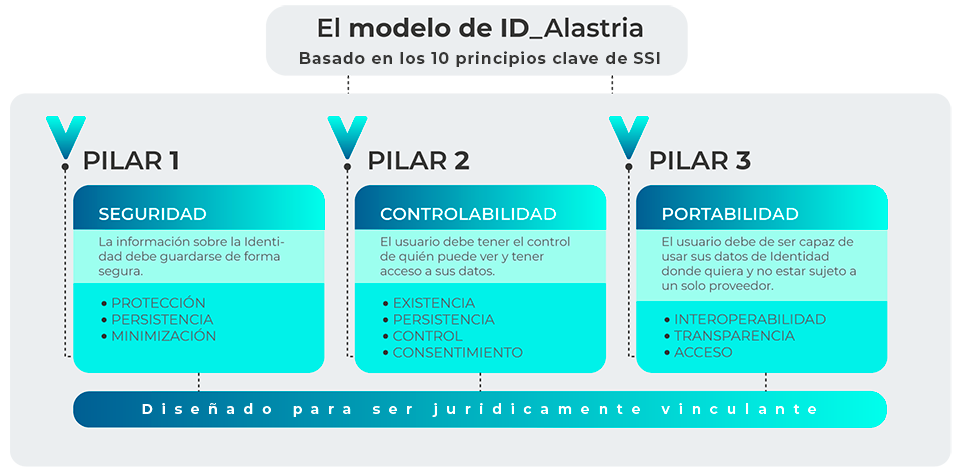
\includegraphics[width=1.0\textwidth]{pilares_alastria.png}
        \caption{Alastria ID model}
        \label{fig:pilares_alastria}
    \end{figure}
                    
    As the figure \ref{fig:pilares_alastria} obtained from the Alastria main website\footnote{https://alastria.io/en/id-alastria/} represents, the Alastria ID model is based in the 10 key principles of the \acrshort{ssi}. It is designed to be legally binding, and its three fundamental pillars are:
    \begin{itemize}
        \item \textbf{Security}: identity information must be kept secure. This means protection, persistence and minimization.
        \item \textbf{Controllability}: the user must have control of who can see and have access to their data. This means existence, persistence, control and consent.
        \item \textbf{Portability}: the user must be able to use their data wherever they want and not be subject to a single provider. This means interoperability, transparency and access.
    \end{itemize}
    
    \subsection{Actors}
        In the model several actors are defined, with different functionalities.
         \begin{itemize}
             \item \textbf{Entity}: Company or organization (legal person). An entity can be one or both:
             \begin{itemize}
                 \item \textbf{Service Provider}: Entity which requests information from a subject, so \textbf{it creates Presentation Requests and receives Presentations}.
                 \item \textbf{Issuer}: It can help anyone to create a new identity. Also this kind of entity can emits certified information about a subject, so \textbf{it creates Credentials}.
             \end{itemize}
             \item \textbf{Subject}: Person (natural or legal) who \textbf{has information certified by an Issuer and sends it to a Service Provider}, so it receives credentials and creates presentations. It is the information owner. This information is saved and controlled from a wallet.
             \item \textbf{Admin}: It is the \textbf{identity} (account) \textbf{that deployed the Smart Contracts}. \textbf{It is only used to create the first entity} (Issuer). \textbf{All other identities must be created by Issuers}.
        \end{itemize}
        In the next figure (\ref{fig:roles-ala}) we can see a visual explanation of the data flow between the different actors.
        \begin{figure}[h]
            \centering
            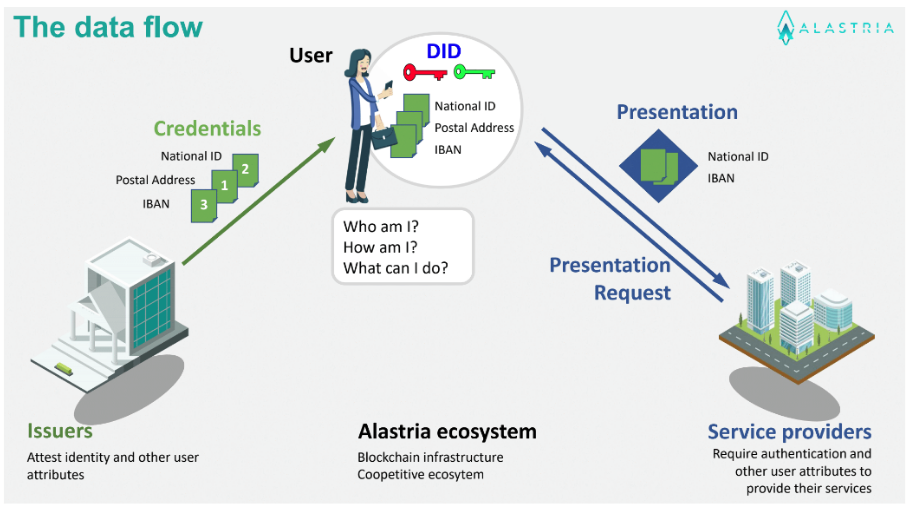
\includegraphics[width=1.0\textwidth]{roles-ala.png}
            \caption{Data flow between different actors in Alastria}
            \label{fig:roles-ala}
        \end{figure}

    \subsection{Alastria ID Specification}
        In this section we are going to see the different objects defined by Alastria for the model.
        \subsubsection{DID}
            As we have seen previously, the \acrfull{dids} are a type of identifier that allows the verification of decentralized identities. It should be noted that all entities, regardless of their role, have a DID that identifies them. At Alastria, the W3C standard is followed with a few minor differences.
            \begin{itemize}
                \item It will include the type of network in which the \acrshort{did} has been registered.
                \item It will also include the blockchain network and the network ID where the \acrshort{did} is registered.
            \end{itemize}
            
            Alastria \acrshort{dids} have the following format (listing \ref{lst:did_format}):
            \lstinputlisting[label={lst:did_format}, caption=DID format]{examples/codeSnippets/did_format.txt}
            Where:
            \begin{itemize}
                \item \textbf{"ala"}: specifies that this is a \acrshort{did} for Alastria.
                \item \textbf{"network"}: specifies the technology used on that network. 
                \item \textbf{"net-id"}: defines the specific Alastria blockchain network instance.
            \end{itemize}
            Possible examples of \acrshort{dids} are (listing \ref{lst:did_ex}):
            \lstinputlisting[label={lst:did_ex}, caption=Examples of DIDs]{examples/codeSnippets/did_examples.txt}

        
    \subsection{Example: Rent a car}
        
    \subsection{Project structure}
    
        \subsubsection{Smart Contracts}
        
        \subsubsection{Node Library}
        
        \subsubsection{Library examples}
        
        \subsubsection{Wallet}

\newpage
\section{Conclusions}
% TODO hacer

\newpage
\section{Future Work}

\newpage
% \nocite{*} % Cita todas las ref (incluidas las no citadas)
\printbibliography[heading=bibnumbered] % Última sección, numerada, para la bibliografía

\end{document}
